\section{Design and Theory}

A velocity field is a function taking as input a state, $q$ and returns a 3 dimensional desired velocity vector $(u,v,w)$.\\ It describes a path (a function of position) as opposed to a trajectory (function of position and time).

\subsection{Spherical field to maintain desired force }
When contact has been made, we suppose that the surface static friction coefficient is high enough to maintain the contact.
Since the arm has a fixed size and does not move, this section will describe a velocity field on the surface of a sphere around the target point with a radius defined by the distance between the CoM of the quadcopter and the tip of the arm.\\
Computing the field on the surface of a sphere is very computationally efficient because we do not have to sample field vectors in the whole 3d space around the point of interest.
First we need to compute the feasible position of the CoM to apply the desired force. 
We know that this position is unique because there is only one vertically stable pitch for a given desired force amplitude. The quadcopter needs to pitch to have a forward velocity because the quadcopter is underactuacted.\\
We can either compute this position analytically or we can use machine learning techniques such as regression to compute the feasible pitch as a function of the desired force. The latter option would require collecting training data from simulations on Gazebo. 
Now we can generate the velocity field on the surface of the sphere to point on the tangent direction of the sphere in the direction of the stable pitch position. \\
This field will have an amplitude proportional to the distance from this point.
The planning strategy we described would also allow us to easily define a desirable range for the yaw angle depending on the type of sensor and on the friction coefficient of the target surface.
Finally, we use a Passive Velocity Field Controller \cite{li1999passive} to follow this field to minimize the loss of kinetic energy to the environment when interacting with the surface.
Now we are going to describe how the spherical field is computed. 
Let us recall that the cartesian to spherical change of variable is defined as
\begin{equation} 
    r = \sqrt{x^2+y^2+z^2}\\ \nonumber 
\end{equation}
\begin{equation}
    \theta = \arccos(\frac{z}{r})\\\nonumber 
\end{equation}
\begin{equation}
    \label{transformation}
    \phi =
    \begin{cases}
        \arctan(\frac{y}{x}), & \text{if $x>0$},\\
        \arctan(\frac{y}{x}) + \pi, & \text{if $x<0$ and $y\geq 0$},\\
        \arctan(\frac{y}{x}) - \pi, & \text{if $x<0$ and $y<0$},\\
        \pi/2, & \text{if $x=0$ and $y>0$},\\
        -\pi/2, & \text{if $x=0$ and $y<0$},\\
        not defined , & \text{if $x=0$ and $y=0$}
    \end{cases}       
\end{equation}  
The jacobian defining the curvature of the sphere for at each point for this transformation is 
\begin{align}
    J = \frac{\partial{(x,y,z)}}{\partial{(r,\phi,\theta)}} \nonumber\\
    J = \begin{bmatrix}
        \sin(\theta)\cos(\phi) & \cos(\theta)\cos(\phi) & -\sin(\phi)\\
        \sin(\theta)\sin(\phi) & \cos(\theta)\sin(\phi) & \cos(\phi)\\
        \cos(\theta) & -\sin(\theta) & 0\\
        \end{bmatrix}
        \label{jacobian}
\end{align}
We can now derive this velocity field in 3 steps:
\begin{enumerate}
    \item Sample a list of point on the surface of the sphere in cartesian coordiate. In Python or Matlab, a meshgrid can be used where we the field will be non zero with \begin{equation} | \sqrt{x^2+y^2+z^2}-R_{sphere}|\leq\epsilon\nonumber \end{equation} where $R_{sphere}$ is the radius of the mounted arm.
    \item For each point in the list, we compute its spherical coordinate according to \ref{transformation} and we compute the jacobian at the point
    \item Let $(\phi_{opt}, \theta_{opt})$ be the desired position on the sphere. For each point $(\phi, \theta)$ on the sphere , we compute the tangeant vector in the the field that will point toward the goal as \\$J(r, \phi, \theta).(\epsilon, \phi_{opt}-\phi, \theta_{opt}-\theta)^T$ using the jacobian defined in \ref{jacobian} 

\end{enumerate}

\subsection{Passive Velocity Field Control of Mechanical Manipulators}
In \cite{li1999passive}, the author explains the advantages of encoding a contour following task using velocity fields. 
He later presents the passive velocity field controller whose objective is to "maintain an energetically passive relation-ship between the manipulator under closed loop control and
its physical environment, while causing the manipulator to perform the desired task." 
We will explain each one of those arguments and relate them to our sensor placement task.
\subsubsection{Velocity fields for planning}
The classical approach to do planning is to encode the task into a timed trajectory $Q:\mathbb R_{\ge 0} \rightarrow G$ where G is the n-dimensional configuration manifold for the manipulator.
Using this strategy, the objective of the controller is to minimize the deviation between $q(t)$ and $Q(t)$ where $q:\mathbb R_{\ge 0} \rightarrow G$ is the actual coordinate representation of the manipulator.
This strategy could be fine if the manipulator was able to never deviate from the timed trajectory defined by Q. However, this is rarely the case and when a deviation occurs, a side effect of this minimization strategy called radial reduction can occur.
\begin{figure}[h!]
    \centering
    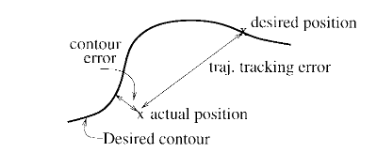
\includegraphics[width=0.48\textwidth]{Images/radialreduction.png}
    \caption{radial reduction from \cite{li1999passive}}
    \label{fig:radialreduction}
\end{figure} 
The author argues that if following the path of the desired trajectory is more important than the timing in which the manipulator follows this trajectory, a strategy based on velocity field is more appropriate because the velocity of the manipulator will only depend on its current position and will be time invariant.  
For the sensor placement task, using a timed trajectory strategy with deviation minimization to reach the contact point may lead the UAV to collide with an obstacle. With our strategy based on potential velocity field, the UAV will not try to shortcut the desired path in case of deviation.

\subsubsection{Passive velocity field controller}
The controller presented in this paper allows storing kinetic energy of the manipulator's actuators in a spring or a flywheel and releasing it when needed so that we can interact with surfaces while minimizing energy loss. This is useful because the UAV has a limited amount of energy stored in its battery and this is one of the main limiting factors for most tasks (including Sensor Placement). \\
To present this concept, the author first define the notion of a passive dynamic system:\\
A dynamic system with input $u \in U$ and output $y \in Y$ is passive with respect to the supply rate 
$s:U \cross Y \rightarrow \mathbb R$, if for any $u: \mathbb R_{\ge 0} \rightarrow U $ and for any $t\geq 0$ the following relation is satisfied:
\begin{align}
    \exists ~ c\in\mathbb R  \nonumber\\
    \int_{0}^{t}s(u(\tau),y(\tau))d\tau \geq -c^2
\end{align}

Let us remember that the work $W$ and power $P$ of a force $F$ on a point mass object with velocity $v$ are defined as
\begin{align}
    P = F.v\\
    W = \int_{0}^{t}P dt
\end{align}

Therefore the supply rate  $s(\tau_{tot},\dot{q})=\tau_{tot}^{T}\dot{q}$ can be seen as the total mechanical power input. Here the input $\tau_{tot}$ is the total force exerted on the manipulator 
and the output $\dot{q}$ is the velocity of the manipulator. 

When considering a feedback system interacting with the environement shown in figure \ref{fig:pvfccontrolloop}, we can decompose $\tau_{tot}=\tau_{e}+\tau$ (where $\tau$ and $\tau_{e}$ are respectively the forces generated by the actuators and the external forces, for example the contact force when touching a surface),
we can derive the power generated by external forces as $s(\tau_{e}\dot{q})=\tau_{e}^T \dot{q}$. 
\begin{figure}[h!]
    \centering
    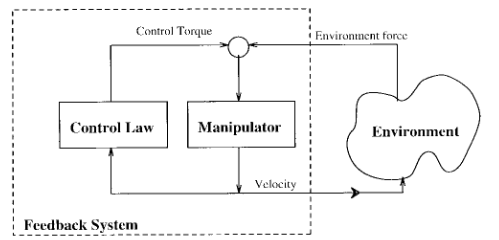
\includegraphics[width=0.48\textwidth]{Images/pvfccontrolloop.png}
    \caption{PVFC loop \cite{li1999passive}}
    \label{fig:pvfccontrolloop}
\end{figure} 
As explained in the paper, a system defined by this supply rate is not passive because obstacles may bring the manipulator to a complete stop for an unbounded amount of time and this loss of kinetic enery cannot be bounded. 
As a result, the passivity relation 
\begin{equation}
    \int_{0}^{t}\tau_{e}^T \dot{q}d\tau \geq -c^2 
\end{equation}
is not valid here because the l.h.s represents the total amount of energy lost to the environment and, as stated before, it cannot be bounded. 
This issue motivates the introduction of an augmented system: a fictitious flywheel is added to the system that acts as an energy storage element.
The dimensionality of the manifold is then increased by one to include the state of the flywheel and this augmented state will be noted as
\begin{equation} 
    \bar{q}=[q_1,...,q_n,q_{n+1}]
\end{equation}
The paper later presents the dynamics of this augmented state and designs a field for the fictitious flywheel such that "the kinetic energy of the augmented system remains constant"

Diverse ways of placing sensors using UAVs have been explored in the past, including but not limited to: 
\begin{itemize}
    \item Direct Placement: Using a fixed arm manipulator on an UAV, we use the force exerted by the thrust of the UAV to provide enough pressure on the tip of the arm to place the sensor on the target point.
    \item Sensor Launching \cite{farinha2020unmanned}: Using the energy stored in a spring, the UAV ejects the sensor at the desired velocity to reach and attach to the target (Unmanned Aerial Sensor Placement for Cluttered Environments). This strategy is very useful when it is not physically possible for a mounted arm to reach the target however it suffers from small payload capacity.
    \item Drop from flight: We simply drop the sensor above the target point. When target accuracy is not a priority and we are aiming at a non-vertical surface and there is no occlusion above the target,  this sensor placement strategy is the most effective. 
\end{itemize}
\begin{figure}[h!]
    \centering
    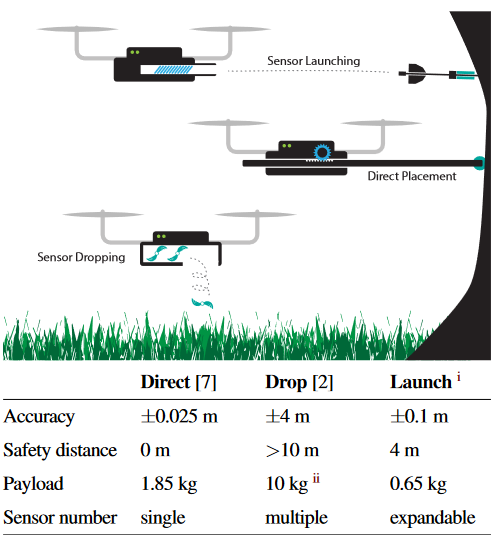
\includegraphics[width=0.48\textwidth]{Images/threeway.png}
    \caption{Different types of sensor placement from \cite{farinha2020unmanned}}
    \label{fig:threeway}
\end{figure}

The characteristics of each one of mentioned methods are shown in \ref{fig:threeway}.
We decided to go through with the Direct Placement strategy because despite its simplicity, it provides good accuracy and is able to place a large variety of payloads.\\

In this section, we will present the field we previously described with illustrations. 
\begin{figure}[h!]
    \centering
    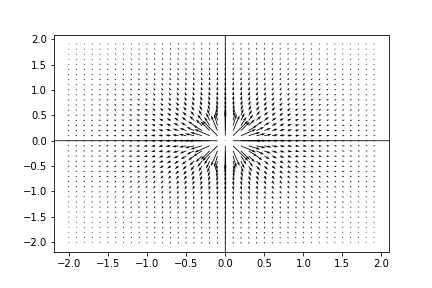
\includegraphics[width=0.48\textwidth]{Images/simplesource.png}
    \caption{Simple Type 1 irrotational source}
    \label{fig:simplesource}
\end{figure}
The field in figure \ref{fig:simplesource} was drawn by computing the gradient of $V_1$ with $(\tilde{{x}_{1}}, \tilde{{x}_{2}}) = (0,0)$.

\begin{figure}[h!]
    \centering
    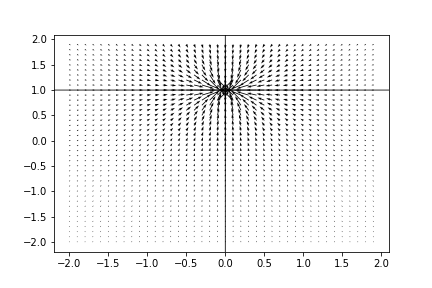
\includegraphics[width=0.48\textwidth]{Images/simplesink01.png}
    \caption{Simple Type 1 irrotational sink}
    \label{fig:simplesink}
\end{figure}
The field in figure \ref{fig:simplesink} is a sink field at $(0,1)$, it is similar to the source field in figure \ref{fig:simplesource} but with opposite sign.

\begin{figure}[h!]
    \centering
    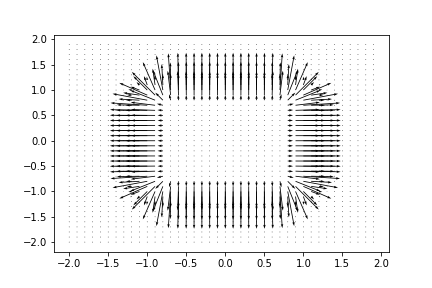
\includegraphics[width=0.48\textwidth]{Images/irrotafromshaping.png}
    \caption{irrotational field from shaping}
    \label{fig:irrotafromshaping}
\end{figure}
The field in figure \ref{fig:irrotafromshaping} has been generated by computing the gradient of the shaping function of a superquadratic: 
\begin{align}
    H=(x_1-\tilde{{x}_{1}})^n+(x_2-\tilde{{x}_{2}})^n \\
    F=\frac{1}{1+(\frac{1}{L}H^{\frac{1}{n}})^m}
\end{align}
As stated in \cite{mcinnes2003velocity}, when $m\gg1$, the edge of the shaping function gets thinner. Higher values of $n$ result in more rectangular shapes whereas $n=2$ describes the shaping function of a sphere.

Both these fields are type 1 irrotational solutions of the Laplace equation.

By adding the irrotational sink from figure \ref{fig:simplesink} and the irrotational field from shaping function in figure \ref{fig:irrotafromshaping} we obtain a good representation in figure \ref{fig:irrotafromshapingwithsink} of what the velocity field will look like when close to the target point. 
\begin{figure}[h!]
    \centering
    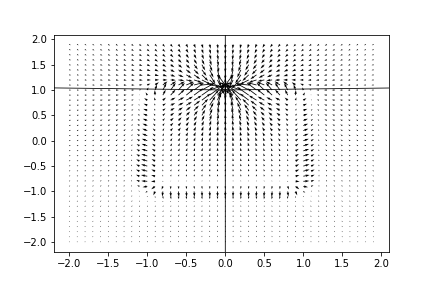
\includegraphics[width=0.48\textwidth]{Images/irrotashapingwithsink.png}
    \caption{irrotational field from shaping with sink}
    \label{fig:irrotafromshapingwithsink}
\end{figure}

The shaping function is mainly used to generate a vortex field around an obstacle, as explained in the paper. It is given by: 
\begin{equation}
    v_2=-\frac{\partial{F}}{\partial{x_2}}e_1 + \frac{\partial{F}}{\partial{x_1}}e_2
\end{equation}
Here, $e_1$ and $e_2$ are an orthonormal basis. \\ 
We can see in figure \ref{fig:rotafromshaping} an example of vortex field around a super quadriatic.
\begin{figure}[h!]
    \centering
    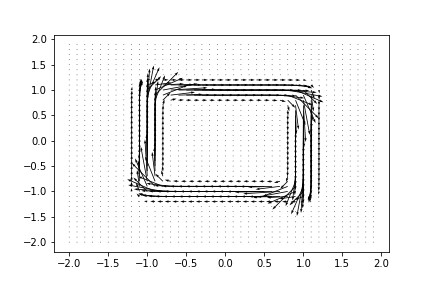
\includegraphics[width=0.48\textwidth]{Images/rotafromshaping.png}
    \caption{Solenoidale field from shaping function}
    \label{fig:rotafromshaping}
\end{figure}

As explained in section 2, after we made contact, we stop using the potential based field and we use the spherical field to maintain 
contact with the desired force.
Figure \ref{fig:spherical} represents an example of such a field where the red point is the optimal position to apply the pressure, the blue arrows are the velocity field vectors and the center of the sphere is the point where the pressure is applied

\begin{figure*}[h!]
    \centering
    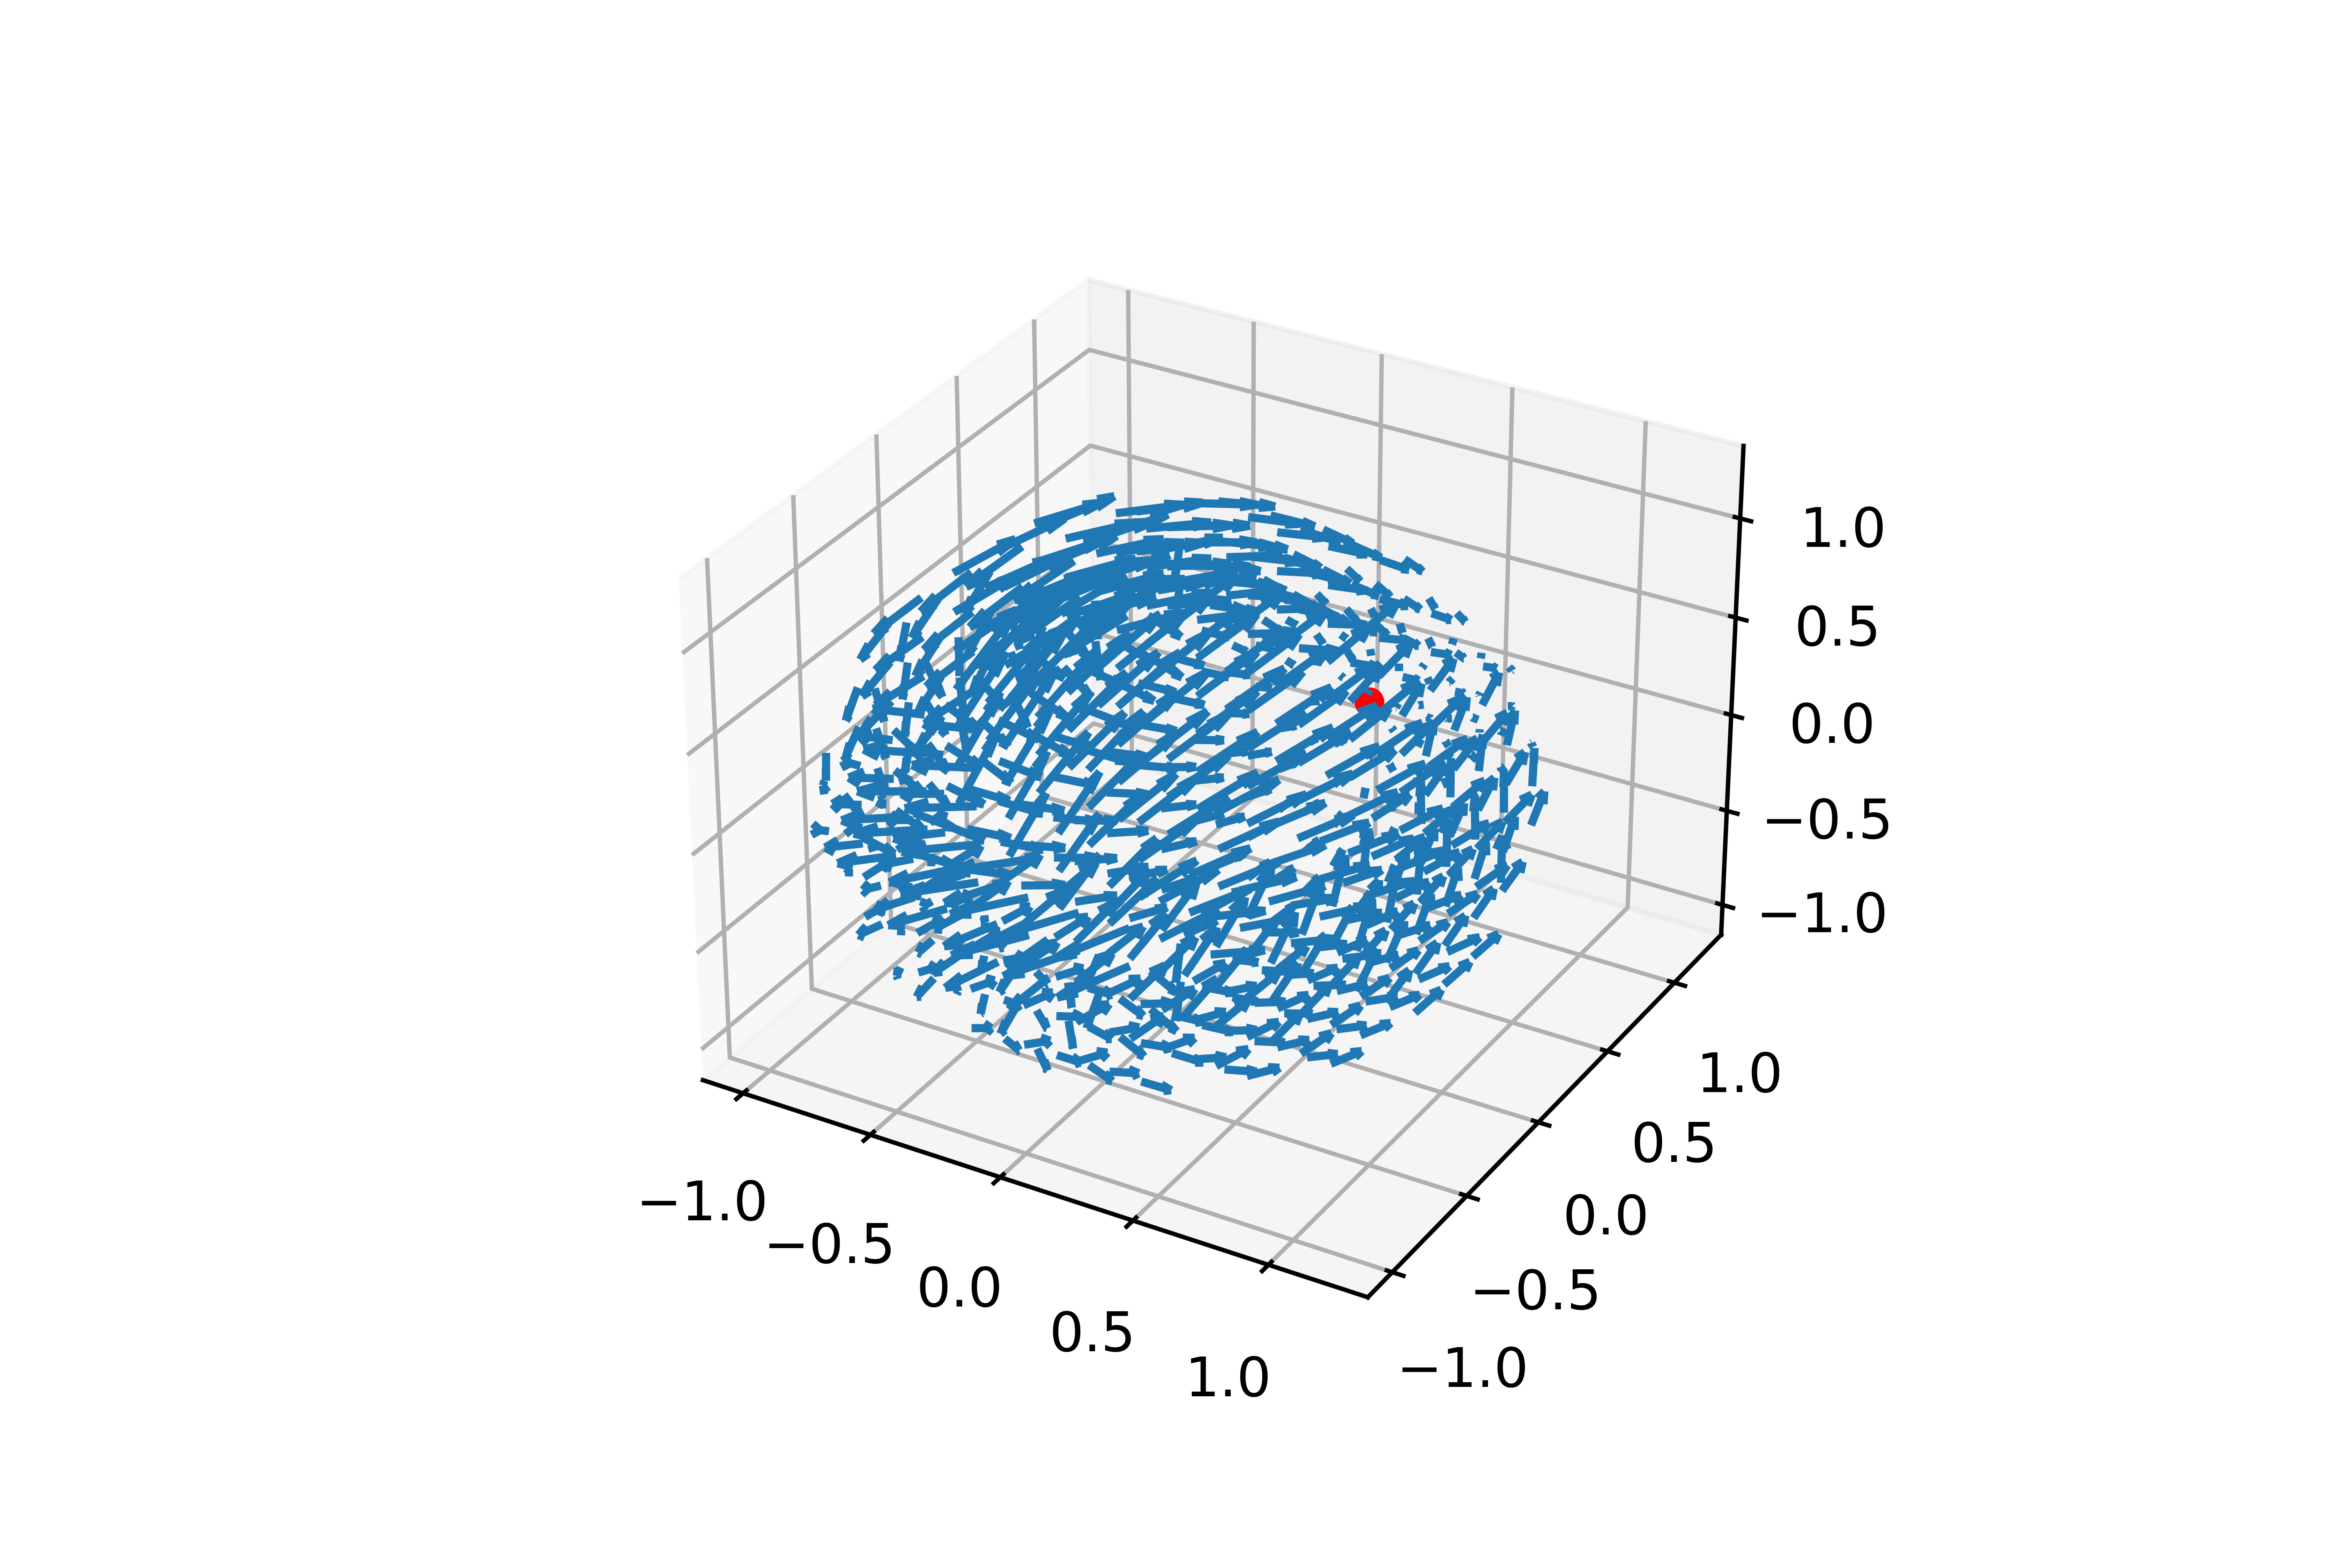
\includegraphics[width=\linewidth]{Images/sphericalfield.png}
    \caption{Spherical contact field}
    \label{fig:spherical}
\end{figure*}
